\documentclass{article}

\usepackage{amsmath}
\usepackage{amssymb}
\usepackage{amsthm}
\usepackage{graphicx}
\usepackage{float}
\graphicspath{ {./images/} }
\usepackage{pdfpages}
\usepackage{hyperref}
\usepackage[danish]{babel}
\usepackage{tikz}
\usepackage{mathtools}

\usepackage{caption}

\usetikzlibrary {angles, quotes, through}
\usetikzlibrary{calc, tikzmark, intersections}

\usepackage[e]{esvect}

\usepackage{tcolorbox}

\newcommand\gap[0]{\ensuremath{\hspace{1cm}}}

\newcommand\vektor[2]{\ensuremath{
    \begin{pmatrix}
        #1\\
        #2
    \end{pmatrix}
}
}

\newcommand\billede[3][1\textwidth]{\begin{figure}[H]
    \caption{#3}
    \includegraphics[width=#1]{#2}\label{#2}
    \centering
\end{figure}}

\newcommand\cel{\ensuremath{^\circ\mathrm{C}}}
\newcommand\grader{\ensuremath{^\circ}}
\newcommand\dx{\:\mathrm{d}x}
\newcommand\ud{\,\mathrm{d}}

\newcommand\lr{\ensuremath{\Leftrightarrow}}
\newcommand{\R}{\ensuremath{\mathbb{R}}}
\newcommand{\C}{\ensuremath{\mathbb{C}}}
\newcommand\dmht[1]{\frac{\partial}{\partial #1}}

\newcommand\inccounter[1]{\setcounter{#1}{\arabic{#1}+1}}
\newcommand\facit[1]{\underline{\underline{#1}}}

\tcbuselibrary{theorems}

\newcounter{opgave}
\newtcbtheorem[use counter=opgave]{opgave}{Opgave}{separator sign none}{}
\newtcbtheorem[number within=opgave, number format=\alph]{del}{Delopgave}%
{theorem style=plain,colframe=white,coltitle=black,fontupper=\itshape}{}
\newtcbtheorem{formel}{Formel}{theorem style=break,colframe=blue!70!white,coltitle=black!90!white,fonttitle=\itshape}{lm}

\newtcbtheorem[number within=section]{eksempel}{Eksempel}{theorem style=plain, colframe=black, colback=white, %
colbacktitle=blue!30!white,coltitle=black!90!white,fonttitle=\itshape}{ex}
\newtcbtheorem[number within=section]{definition}{Definition}{theorem style=plain, colframe=black, colback=white, boxrule=0.25mm, sharp corners=all,%
colbacktitle=blue!30!white,coltitle=black!90!white,fonttitle=\bfseries}{df}

\newtcbtheorem[number within=section]{theorem}{Sætning}{sharp corners=all, theorem style=plain, colframe=black, colback=white,%
colbacktitle=blue!30!white,coltitle=black!90!white,fonttitle=\bfseries, boxrule=0.25mm}{th}

\newtcbtheorem[number within=section]{lemma}{Lemma}{sharp corners=all, theorem style=plain, colframe=black, colback=white,%
colbacktitle=blue!30!white,coltitle=black!90!white,fonttitle=\bfseries, boxrule=0.25mm}{lm}


\usepackage{caption}

\usetikzlibrary {angles, quotes, through}

\usepackage[e]{esvect}

%\synctex=1

\title{Eksamensnoter}
\author{Ricardt Riis}

\begin{document}

\maketitle

\textbf{Meningen med materialet er som disposition til mundtlig eksamen}

\tableofcontents

\section*{Introduktion}
I det følgende vil overskriften angive hvilket spørgsmål der svares på. Da det
er bedst at svare på begge spørgsmål "samtidigt" eller i det mindste have en
nogenlunde flydende overgang mellem de to spørgsmål, virker det gavnligst at
beskrive spørgsmålene, og dernæst under \textit{EN} overskrift besvare
spørgsmålene.\\
Bemærk desuden, at jeg kun har ringe forståelse af hvad Sætning og Definition
betyder i streng matematisk konstekst.

\begin{tcolorbox}
	\section{Funktioner}
	\tcblower
	\begin{enumerate}
		\item Giv en præsentation af en selvvalgt del af teorien for vektorfunktioner.
		\item Brug vektorfunktioner til at bestemme de afledte af de trigonometriske funktioner.
	\end{enumerate}
\end{tcolorbox}
Her kan man komme ind på følgende:
\begin{itemize}
	\item Funktioner tager et input, og laver et output.
	\item For vektorfunktioner gælder at deres signatur er
		\[
			\mathbb{R} \rightarrow \mathbb{R}^2.
		\] 
	\item Vektorfunktioner skrives
		\[
			\vec{v}(t).
		\] 
	\item $t$ kaldes normalt \texttt{parameterværdi}.
	\item Præsenteres en vektorfunktion grafisk, benyttes en banekurve.\\
		\textit{Bemærk}: En banekurve viser ikke alt ved en vektorfunktion. Fx.
		er banekurverne for $\vektor{t^3}{t^3}$ og $\vektor{t}{t}$ de samme.
	\item Den afledede af en vektorfunktion kan bestemmes således
		\[
			\vec{v}\,'(t) = \vektor{x(t)}{y(t)}' = \vektor{x(t)'}{y(t)'}
		\] 
		\textit{I det følgende vil afledte funktioner skrives således}
		\[
			\dot{\vec{v}}(t) = {\vektor{x(t)}{y(t)}}'
		\] 
	\item Den afledede beskriver retningsvektoren for tangenten til en bestemt
		parameterværdi.

	\item Den afledede kaldes også hastighedsvektoren
	\item Dermed kan farten bestemmes ved længden af hastighedsvektoren
		\[
			\text{fart}(\vec{v}) = \left|\dot{\vec{v}}\right|
		\] 
	\item Se mere viden om vektorer i afsnit om vektorer.
\end{itemize}

\begin{definition}{Cosinus, sinus og tangens}{}
	Cosinus, $\cos$, sinus, $\sin$, og tangens, $\tan$, defineres ud fra
	enhedscirklen, der har radius 1.
	\begin{center}
	\begin{tikzpicture}[scale=2.0]
		\coordinate (A) at (0, 0);
		\coordinate (B) at (0.8660254037844387, 0);
		\coordinate (C) at (0.8660254037844387, 0.5);
		\coordinate (E) at (1, 0.5773502691896257);
		\coordinate (D) at (1, 0);
		\draw (A) -- (B) node [midway, below] {$\cos{t}$};
		\draw (C) -- (B) node [midway, left] {$\sin{t}$};
		\draw (A) -> (C) node [midway, above] {$\vec{r}$};
		\draw[dotted, thick] (C) -- (E);
		\draw[dotted, thick] (D) -- (E) node [midway, right] {$\tan{t}$};
		\draw pic [draw] {angle = B--A--C};
		\node [above] at (0.30, -0.025) {$t$};

		\draw[->,thick] (-1.5,0)--(1.5,0) node[right]{$x$};
		\draw[->,thick] (0,-1.5)--(0,1.5) node[above]{$y$};
		\node [draw,circle through=(D)] at (A) {};
	\end{tikzpicture}
	\end{center}
\end{definition}

\begin{lemma}{Idiotformlen}{idformel}
	\( \cos^2{t} + \sin^2{t} = 1 \)	
\end{lemma}

\begin{definition}{}{}
	\[
		\vec{r}(t) = \vektor{\cos{t}}{\sin{t}}
	\] 
\end{definition}

\begin{theorem}{Afledte cosinus og sinus}{cossindiff}
	\begin{align*}
		\cos' &= -\sin\\
		\sin' &= \cos
	\end{align*}
\end{theorem}

\textbf{Bevis:}
Det ønskes at finde $\dot{\vec{r}}(t)$, da vi i så fald kan bevise sætning
\ref{th:cossindiff}.

\smallskip

Det vides om $\vec{r}$ at den bevæger sig langs enhedscirklens periferi. Dvs.
at for hver omgang $\vec{r}$ bevæger sig omkring periferien, har punktet som
stedvektoren $\vec{r}$ beskriver bevæget sig $2\pi$. Da perioden for $\vec{r}$
også er $2\pi$ ved vi om farten af $\vec{r}$
\[
	|\dot{\vec{r}}(t)| = 1.
\] 
\textit{Bemærk, at længden af $\vec{r}$ også er 1 (jf. lemma \ref{lm:idformel}).}\\
Det vides om tangenter til punkter på en cirkel står ret på stedvektoren til
punktet. Dermed gælder
\[
	\dot{\vec{r}} = \hat{\vec{r}}.
\]
Derfor
\begin{align*}
	\dot{\vec{r}} = {\vektor{\cos}{\sin}} &= \widehat{\vektor{\cos}{\sin}} = \hat{\vec{r}}\\
						\vektor{\cos'}{\sin'}	&= \vektor{-\sin}{\cos}.
\end{align*}
Da lighedstegnet gælder koordinatvis, er beviset gennemført.

\begin{lemma}{Tangens}{tan}
	\(
		\tan = \frac{\sin}{\cos}
	\) 
\end{lemma}

\begin{theorem}{Afledede tangens}{difftan}
	\(
		\tan' = \tan^2 + 1
	\) 
\end{theorem}

\textbf{Bevis:}
\begin{align*}
	\tan' &= \left(\frac{\sin}{\cos}\right)'\\
		  &= \left(\sin \cdot \frac{1}{\cos}\right)'\\
		  &= \cos \cdot \frac{1}{\cos} + \sin \cdot \left(\frac{1}{\cos}\right)'\\
		  &= 1 + \sin \cdot \left(-\frac{1}{\cos^2}\right) \cdot (-\sin)\\
		  &= 1 + \frac{\sin^2}{\cos^2}\\
		  &= \tan^2 + 1
\end{align*}

\begin{tcolorbox}
	\section{Funktioner}
	\tcblower
	\begin{enumerate}
		\item Giv en præsentation af en selvvalgt del af teorien for plus- og gangefølger.
		\item Bevis at to gangefølger altid giver anledning til en potenssammenhæng.
	\end{enumerate}
\end{tcolorbox}

%\section{Funktioner}
\begin{itemize}
	\item Plusfølger lægger til, gangefølger ganger.
	\item Plusfølger gentaget = gange, den anden exponential
	\item Logaritmer laver gange om til plus
	\item Stjæl fra Katrine.
\end{itemize}

\begin{theorem}{Logaritme laver gange om til plus}{loggangeplus}
	\[\log_A{B \cdot C} = \log_AB + \log_AC\]
\end{theorem}
\textbf{Bevis:}
\begin{align*}
	\log_A{B \cdot C} &= \log_AB + \log_AC \iff\\
	A^{\log_A{B \cdot C}} &= A^{\log_AB + \log_AC}\\
						  &= A^{\log_AB} \cdot A^{\log_AC} \iff\\
	B \cdot C &= B \cdot C
\end{align*}

\begin{theorem}{Logaritmeregneregel}{}
	$\log_AB^C = C \cdot \log_AB$
\end{theorem}
\textbf{Bevis:}
\begin{align*}
	\log_AB^C &= \log_A{B \cdot B \cdots B}\\
			  &= \log_A{B} + \log_A{B} + \cdots + \log_A{B}\\
			  &= C \cdot \log_AB
\end{align*}

\begin{theorem}{Logaritmeregneregel}{logswap}
	$A^{\log_BC} = C^{\log_BA}$.
\end{theorem}
\textbf{Bevis:}
\begin{align*}
	A^{\log_BC} &= C^{\log_BA}\\
	B^{\log_B{A^{\log_BC}}} &= B^{\log_B{C^{\log_BA}}}\\
	B^{\log_BC \cdot \log_B{A}} &= B^{\log_BA \cdot \log_B{C}}
\end{align*}

\begin{definition}{Plusfølge}{}
	En plusfølge lægger altid et bestemt tal til for hvert skridt i følgen.
\end{definition}

\begin{definition}{Gangefølge}{}
	En gangefølge gange altid et bestemt tal for hvert skridt i følgen.
\end{definition}

\begin{figure}[H]
	\centering
	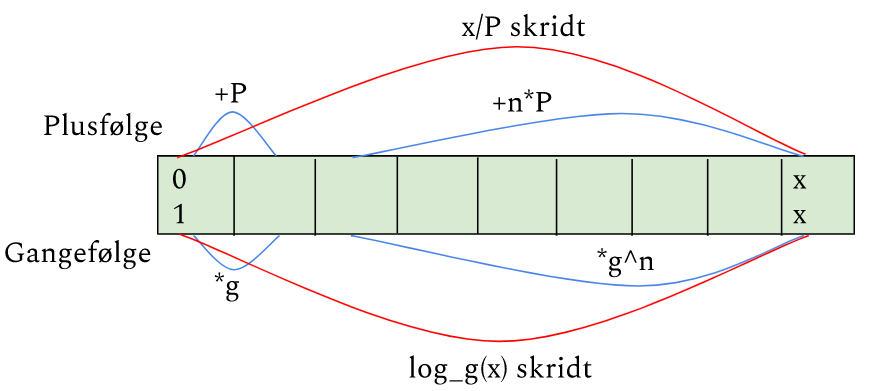
\includegraphics[width=0.8\textwidth]{plus_og_gange}
\end{figure}

\begin{theorem}{Gangeføĺge - Gangefølge}{}
	To gangefølger giver altid anledning til en potenssammenhæng.
	\[
		y = \frac{d}{c^{\log_{Px}{Py}}}\cdot x^{\log_{Px}{Py}}
	\]
\end{theorem}

\begin{align*}
	x_n &= c\cdot Px^n\\
	y_n &= d\cdot Py^n\\
	\intertext{$y$ ønskes fundet ud fra vilkårlig $x$. Dermed ønskes $n$ 
	fundet}
	x &= c\cdot Px^n\\
	\log_{Px}{x}-\log_{Px}{c} &= n\\
	n &= \log_{Px}{\frac{x}{c}}\\
	\intertext{Dette kan sættes ind i $y$ funktionen}
	y &= d\cdot Py^{\log_{Px}{\frac{x}{c}}}\\
	&= d\cdot \frac{x}{c}^{\log_{Px}{Py}}\gap\text{Bevis regneregel}\\
	&= \frac{d}{c^{\log_{Px}{Py}}}\cdot x^{\log_{Px}{Py}}
\end{align*}

\begin{figure}[H]
	\centering
	\caption{En grafisk fremstilling af ovenstående}
	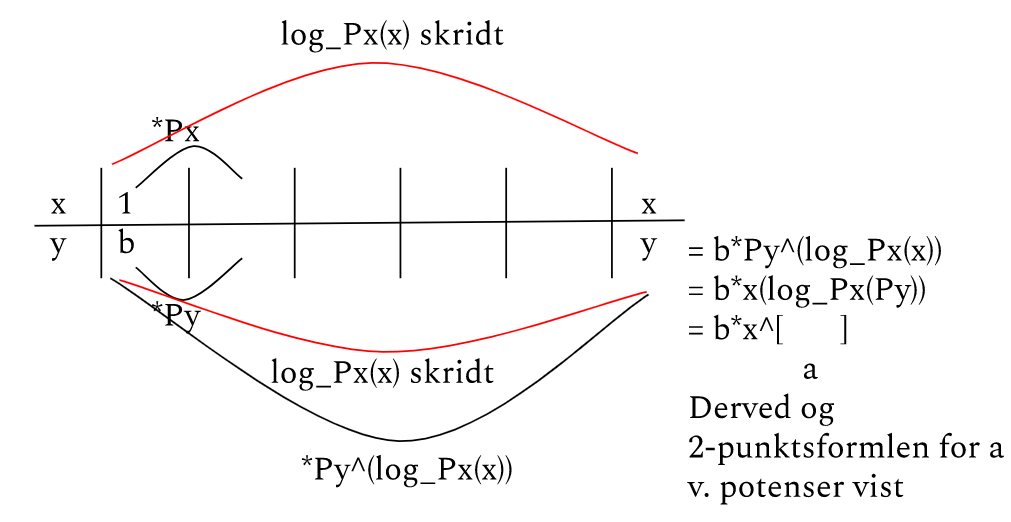
\includegraphics[width=0.8\textwidth]{gangegange}
\end{figure}

\section{Funktioner}
\subsection{Giv en præsentation af en selvvalgt del af teorien for funktioner 
af to variable}
\begin{itemize}
	\item Maskiner, som en variabel
	\item Partiel afledning
	\item Stationære punkter.
\end{itemize}

\subsection{Adled formlen for hældningen af regressionslinjen ved mindste 
kvadraters metode} 
\begin{itemize}
	\item Opskriv KS
	\item Opskriv KS(a), $KS'(a) = 0$
	\item Vilkårligt punkt
	\item $\dmht{a}KS(a, b)$, $\dmht{b}KS(a, b)$
	\item Sæt b lig nul.
	\item Vind
\end{itemize}

\begin{tcolorbox}
	\section{Differential- og integralregning}
	\tcblower
	\begin{enumerate}
		\item Giv en præsentation af en selvvalgt del af teorien for diskret analyse.
		\item Bevis mindst en regneregel for diskret differentiation.
	\end{enumerate}
\end{tcolorbox}
\begin{itemize}
	\item I diskret analyse benyttes talfølger; i stedet for tal funktioner.
	\item For at gøre notationen af uendeligt lange talfølger nemmere, kan man benytte sig af funktionsnotation
		\[
			f(x), x\in\mathbb{N}.
		\]
		\begin{eksempel}{Indeksering}{}\\
			Hvis $f$ defineres ved talfølgen $1, 3, 5, 4, 9$, så vil
			\[
				f(3) = 5,
			\] 
			og $f(2.5)$ være udefineret.
		\end{eksempel}
	\item Der indføres desuden en anden potensfunktion
		\[
			x^{\overline{n}} = \frac{x!}{(x-n)!}
		\] 
		\begin{eksempel}{x i n-streg}{}
			$
				7^{\overline{4}} = 7 \cdot 6 \cdot 5 \cdot 4.
			$ 
		\end{eksempel}
	\item Det kaldes at differentiere når man trækker nabo-elementer fra hinanden
		\[
			\Delta f: [2, 2, -1, 5].
		\] 
	\item Det kan skrives med symboler
		\begin{definition}{Differentiation}{diff}
			$
				\Delta f(x) = f(x + 1) - f(x).
			$ 
		\end{definition}
	\item Man kan desuden definere integration
		\begin{definition}{Integration}{dint}
			\[
				F(x_0) = \sum f(x_0) = \sum_{-\infty}^{x_0} f(x) 
			\]
		\end{definition}
	\item Det følger let at følgende gælder
		\begin{theorem}{Integralregningens hovedsætning}{main}
			\[
				\sum_a^b f(x) = F(b + 1) - F(a)
			\]
		\end{theorem}
\end{itemize}

\begin{theorem}{Produktregel for differentiation}{produktdiff}
	\[
		\Delta (f \cdot g)(x) = \Delta f(x) \cdot g(x) + f(x + 1) \cdot \Delta g(x)
	\] 
\end{theorem}
\textbf{Bevis:}
\begin{align*}
	\Delta (f \cdot g)(x) &= \Delta (f(x) \cdot g(x))\\
						  &= f(x + 1) \cdot g(x + 1) - f(x) \cdot g(x)\\
						  &= f(x + 1) \cdot (g(x) + \Delta g(x)) - (f(x + 1) - \Delta f(x)) \cdot g(x)\\
						  &= f(x + 1) \cdot g(x) + f(x + 1) \cdot \Delta g(x) \\
						  &\gap- f(x + 1) \cdot g(x) + \Delta f(x) \cdot g(x)\\
						  &= \tcbhighmath{f(x + 1) \cdot g(x)} + f(x + 1) \cdot \Delta g(x) \\
						  &\gap\tcbhighmath{- f(x + 1) \cdot g(x)} + \Delta f(x) \cdot g(x)\\
						  &= f(x + 1) \cdot \Delta g(x) + \Delta f(x) \cdot g(x)
\end{align*}

\begin{theorem}{Differentiation af $x^{\overline{n}}$}{diffxn}
	Givet konstant $n$ og variabel $x$ gælder
	\[
		\Delta x^{\overline{n}} = n \cdot x^{\overline{n-1}}.
	\]
\end{theorem}
\textbf{Bevis:}
\begin{align*}
	\Delta x^{\overline{n}} &= (x+1)^{\overline{n}} - x^{\overline{n}}\\
	&= (x+1) \cdot x^{\overline{n-1}} - x^{\overline{n-1}} \cdot (x - (n-1))\\
\intertext{Det er vigtigt at indse hvorfor den sidste faktor er $(x - (n-1)$.}
	&= (x + 1 - x + (n - 1)) \cdot x^{\overline{n-1}}\\
	&= n \cdot x^{\overline{n-1}}
\end{align*}

\section{Differential- og integralregning}
\subsection{Giv en præsentation af en selvvalgt del af teorien for 
differential- og integralregning}
\begin{itemize}
	\item Sekanthældning
	\item Grænseværdier
	\item Tangenthældninger
\end{itemize}

\subsection{Bevis mindst en regneregel for differentiation}
\begin{itemize}
	\item Kædereglen
	\item $(\ln{x})'$
	\item $(x^n)'$, hvor $n\in\C$
\end{itemize}

\section{Differential- og integralregning}
\subsection{Giv en præsentation af en selvvalgt del af teorien for 
differential- og integralregning}
\begin{itemize}
	\item Sekanthældning
	\item Grænseværdier
	\item Integraler
\end{itemize}

\subsection{Redegør for sammenhængen mellem stamfunktion og areal}
% TODO: tjek fortegn
\begin{itemize}
	\item Bevis $\int_a^b f dx = F(b)-F(a)$ 
\begin{align*}
	\intertext{Antag $f$ kontinuert}
	\intertext{Antag en arealfunktion for $f$, $A(x)$, som finder areal mellem
	0 og $x$. Ønskes nu arealet af et interval bestemt, kan man finde det ved}
	\int_{x_0}^x f(x) dx &= A(x) - A(x_0)\gap\text{Overbevisende ved graf}\\
	\intertext{Dette areal kan også estimeres ved $f$, som dog giver en mindre
	fejl, $E$}
	A(x) - A(x_0) &= f(x_0)\cdot (x-x_0) + E\\
	f(x_0) &= \frac{A(x)-A(x_0)}{x-x_0} - \frac{E}{x-x_0}\\
	 &= d_A(x) - \frac{E}{x-x_0}\\
	 \intertext{Hvis det kan vises at $\frac{E}{x-x_0}$ går mod nul når $x$ går
	 mod $x_0$, så er $A' = f$. Det vides om $\frac{E}{x-x_0}$}
	\frac{E}{x-x_0} &\le \frac{(x-x_0)\cdot (f(x_0+t_{max})-f(x_0+t_{min}))}
	{x-x_0}\\
	&=f(x_0+t_{max})-f(x_0+t_{min})
\end{align*}
	\item Herfra burde det være muligt at bevise færdig.
\end{itemize} 

\section{Differensligninger}
\subsection{Giv en præsentation af en selvvalgt del af teorien for differensligninger}
\begin{itemize}
	\item Løsning er talfølge
\end{itemize}
\subsection{Udled en løsningsformel til en selvvalgt type differensligning}
\begin{itemize}
	\item Tal også noget om $\Delta f(x) = r\cdot  f(x)+p$
\end{itemize}

\section{Binomial}
\subsection{Giv en præsentation af selvvalgt del af teorien for sandsynlighedsregning med fokus på 
binomialfordelingen}
\begin{itemize}
	\item Tæthedsfunktioner
	\item Bernoulli
	\item Binomialfordeling: Mange bernoulli
	\item K(n,r)
		\[
			K(n + 1, r) = K(n, r-1) + K(n, r)
		\]
\end{itemize}


Løs K(n,r) ved at indse at der differentieres.

\section{Statistik}
\subsection{Giv en præsentation af en selvvalgt del af teorien for hypotesetest}
\begin{itemize}
	\item Nulhypotese
	\item Hvornår er hvad rigtigt?
	\item Bevis
		\[
			P(p\in[\hat p \pm 2\cdot\sqrt{\frac{\hat p\cdot(1-\hat p)}{n}}]) \approx 95\%
		\]
	\item Ved $\hat p = \frac{X}{n}$, og $X \in $
\end{itemize}

\section{Transformationer}
\begin{itemize}
	\item Flytning (x, y)
	\item Strækning (x, y)
	\item $e^{-\frac{1}{2}x^2}$
	\item Tæthedsfunktioner
	\item Areal
	\item Skaler langs y.
	\item Strækning langs x, konsekvenser
	\item Middelværdi
\end{itemize}

\begin{tcolorbox}
	\section{Vektorer}
	\tcblower
	\begin{enumerate}
		\item Giv en præsentation af en selvvalgt del af teorien for vektorer.
		\item Gør rede for skalarproduktet og måder at beregne dette på.
	\end{enumerate}
\end{tcolorbox}

\begin{itemize}
	\item Vektorer er abstrakte pile, man kan lægge dem sammen og trække fra.
		Vektoren starter ikke et bestemt sted
	\item Består af en længde og en retning
\end{itemize}
\begin{theorem}{Skalarprodukt ved længder}{scalar_prod_len_vec}
	En regneoperation der ganger to vektorer sammen og giver et tal, som givet
	tre vektorer af samme dimension $\vec{a}$, $\vec{b}$ og $\vec{c}$ opfylder
	\begin{enumerate}
		\item $\vec{c} \cdot (\vec{a} + \vec{b}) = \vec{c} \cdot \vec{a} + \vec{c} \cdot \vec{b}$,
		\item $\vec{a} \cdot \vec{b} = \vec{b} \cdot \vec{a}$, og
		\item $\vec{a}\,^2 = |\vec{a}|^2$,
	\end{enumerate}
	kan kun give
	\[
		\vec{a} \cdot \vec{b} = \frac{|\vec{a} + \vec{b}|^2 - |\vec{a}|^2 - |\vec{b}|^2}{2}.
	\] 
	\textit{Operationen kaldes også prikprodukt}.
\end{theorem}
\textbf{Bevis:}
\begin{align*}
	(\vec{a} + \vec{b})^2 &= (\vec{a} + \vec{b}) \cdot (\vec{a} + \vec{b})\\
						  &= (\vec{a} + \vec{b}) \cdot \vec{a} + (\vec{a} + \vec{b}) \cdot \vec{b}\\
						  &= \vec{a} \cdot (\vec{a} + \vec{b}) + \vec{b} \cdot (\vec{a} + \vec{b})\\
						  &= \vec{a}\,^2 + \vec{a} \cdot \vec{b} + \vec{b} \cdot \vec{a} + \vec{b}\,^2\\
						  &= \vec{a}\,^2 + 2 \cdot \vec{a} \cdot \vec{b} + \vec{b}\,^2\\
						  \intertext{Der omarrangeres}
	\vec{a} \cdot \vec{b} &= \frac{(\vec{a} + \vec{b})^2 - \vec{a}\,^2 - \vec{b}\,^2}{2}\\
						  &= \frac{|\vec{a} + \vec{b}|^2 - |\vec{a}|^2 - |\vec{b}|^2}{2}
\end{align*}

\begin{theorem}{Skalarprodukt ved dekomposanering af vektorer}{}
	Givet to vektorer $\vec{a}$ og $\vec{b}$, som kan dekomposaneres til $\vektor{a_1}{a_2}$ og $\vektor{b_1}{b_2}$, så gælder
	\[
		\vec{a} \cdot \vec{b} = a_1 \cdot b_1 + a_2 \cdot b_2.
	\] 
\end{theorem}
\textbf{Bevis:}
\begin{align*}
	\vec{a} \cdot \vec{b} &= \frac{|\vec{a} + \vec{b}|^2 - |\vec{a}|^2 - |\vec{b}|^2}{2}\\
						  &= \frac{(\vec{a} + \vec{b})_1^2 + (\vec{a} + \vec{b})_2^2 - (\vec{a}_1^2 + \vec{a}_2^2) - (\vec{b}_1^2 + \vec{b}_2^2)}{2}\\
						  &= \frac{(\vec{a}_1 + \vec{b}_1)^2 + (\vec{a}_2 + \vec{b}_2)^2 - (\vec{a}_1^2 + \vec{a}_2^2) - (\vec{b}_1^2 + \vec{b}_2^2)}{2}\\
						  &= \frac{\vec{a}_1^2 + 2 \cdot \vec{a}_1 \cdot \vec{b}_1 + \vec{b}_1^2 + \vec{a}_2^2 + 2 \cdot \vec{a}_2 \cdot \vec{b}_2 + \vec{b}_2^2 - (\vec{a}_1^2 + \vec{a}_2^2) - (\vec{b}_1^2 + \vec{b}_2^2)}{2}\\
						  &= \frac{2 \cdot \vec{a}_1 \cdot \vec{b}_1 + 2 \cdot \vec{a}_2 \cdot \vec{b}_2}{2}\\
						  &= \vec{a}_1 \cdot \vec{b}_1 + \vec{a}_2 \cdot \vec{b}_2
\end{align*}

\begin{theorem}{Skalarprodukt ved vinkel}{}
	Givet to vektorer $\vec{a}$ og $\vec{b}$, og vinklen mellem disse $v$, gælder
	\[
		\vec{a} \cdot \vec{b} = |\vec{a}| \cdot |\vec{b}| \cdot \cos{v}.
	\] 
\end{theorem}
\textbf{Bevis:}
Det er givet, at cosinusrelationen gælder
\[
	c^2 = a^2 + b^2 - 2 \cdot a \cdot b \cdot \cos{\gamma}.
\] 
\shorthandoff{"}
\begin{center}
\begin{tikzpicture}
	\coordinate (A) at (0, 0);
	\coordinate (B) at (3, 0);
	\coordinate (C) at (5, 2);
	\draw (A) -- (B) node [midway, below=1] {a};
	\draw (C) -- (B) node [midway, below=1] {b};
	\draw (A) -- (C) node [midway, above=1] {c};
 	\draw pic ["$\gamma$", draw] {angle = C--B--A};
\end{tikzpicture}
\end{center}

Der konstrueres en trekant så $c^2$ er $|\vec{a} + \vec{b}|^2$ og $a^2$ er
$|\vec{a}|^2$ og $b^2$ er $|\vec{b}^2|$.
\smallskip

\begin{center}
\begin{tikzpicture}
	\coordinate (A) at (0, 0);
	\coordinate (B) at (3, 0);
	\coordinate (C) at (5, 2);
	\draw[->] (A) -> (B) node [midway, below=1] {$\vec{a}$};
	\draw[->] (B) -> (C) node [midway, below=1] {$\vec{b}$};
	\draw[] (A) -> (C) node [midway, above=1] {$\vec{a} + \vec{b}$};
	\draw[dashed] (B) -- (5,0) coordinate (D);
 	\draw pic ["$\gamma$", draw] {angle = C--B--A};
 	\draw pic ["$v$", draw] {angle = D--B--C};
\end{tikzpicture}
\end{center}
\shorthandon{"}

I denne trekant vil $\gamma$ være givet ved $180 - v$. Dvs. at udtrykket for
$|\vec{a} + \vec{b}|^2$ kan indsættes i sætning \ref{th:scalar_prod_len_vec}.
Da fås
\begin{align*}
	\vec{a} \cdot \vec{b} &= \frac{|\vec{a}|^2 + |\vec{b}|^2 - 2 \cdot |\vec{a}| \cdot |\vec{b}| \cdot \cos{(180 - v)} - |\vec{a}|^2 - |\vec{b}|^2}{2}\\
						  &= \frac{- 2 \cdot |\vec{a}| \cdot |\vec{b}| \cdot \cos{(180 - v)}}{2}\\
						  &= -|\vec{a}| \cdot |\vec{b}| \cdot \cos{(180 - v)}\\
						  &= |\vec{a}| \cdot |\vec{b}| \cdot \cos{v}.
\end{align*}

\begin{tcolorbox}
	\section{Vektorer}
	\tcblower
	\begin{enumerate}
		\item Giv en præsentation af en selvvalgt del af teorien for vektorer.
		\item Bevis projektionsformlen og gør rede for, hvordan den kan bruges
			i forbindelse med regression eller afstand mellem punkt og linje.
	\end{enumerate}
\end{tcolorbox}

\begin{itemize}
	\item Kør ovenstående
	\item Bevis projektionsformlen
	\item Afstand mellem punkt og linje (mums)
	\item Regression hvis der er tid
\end{itemize}

\section{Annuiteter}
\begin{itemize}
	\item Tænkning kræves
\end{itemize}

\end{document}
